% V-SIL — 4 diapositivas para la Agencia Nacional del Espectro (ANE)
% Audiencia: expertos en espectro y RF, no en ingeniería de software.
% Compilar: latexmk -pdf V-SIL_ANE.tex
%
% Cada diapositiva es un único tikzpicture con coordenadas en mm sobre el
% área útil (142 x 66 mm, origen arriba a la izquierda, y hacia abajo negativo).
\documentclass[aspectratio=169,10pt]{beamer}

\usepackage[utf8]{inputenc}
\usepackage[T1]{fontenc}
\usepackage[sfdefault,lf,scaled=.95]{FiraSans}
\usepackage{fontawesome5}
% mapas de fuentes explícitos (instalaciones TeX sin updmap)
\pdfmapfile{+fontawesome5.map}
\pdfmapfile{+fira.map}
\usepackage{tikz}
\usetikzlibrary{arrows.meta,shapes.geometric,calc}

% ---------- Paleta ----------
\definecolor{navy}{HTML}{0B2545}
\definecolor{ink}{HTML}{1F2937}
\definecolor{muted}{HTML}{6B7280}
\definecolor{line}{HTML}{D1D5DB}
\definecolor{paper}{HTML}{F5F7FA}
\definecolor{design}{HTML}{3B5BA9}   % definir / diseño
\definecolor{designbg}{HTML}{E6ECF8}
\definecolor{sil}{HTML}{0F7C74}      % pruebas en software (SIL)
\definecolor{silbg}{HTML}{DDF1EE}
\definecolor{synth}{HTML}{C77A12}    % señales sintéticas / SDR simulado
\definecolor{synthbg}{HTML}{FCEFD8}
\definecolor{hil}{HTML}{B23A3A}      % hardware real
\definecolor{hilbg}{HTML}{F8E1E1}
\definecolor{gate}{HTML}{2E7D32}     % compuerta automática
\definecolor{gatebg}{HTML}{E3F2E4}
\definecolor{human}{HTML}{8E3B8E}    % compuerta humana
\definecolor{humanbg}{HTML}{F4E6F4}

% ---------- Tema ----------
\setbeamertemplate{navigation symbols}{}
\setbeamercolor{normal text}{fg=ink,bg=white}
\setbeamercolor{structure}{fg=navy}
\setbeamersize{text margin left=9mm,text margin right=9mm}

\setbeamertemplate{frametitle}{%
  \nointerlineskip
  \begin{beamercolorbox}[wd=\paperwidth,ht=15mm,dp=0mm,leftskip=9mm,rightskip=9mm]{}
    \vskip3.4mm
    {\scriptsize\color{sil}\bfseries\MakeUppercase{\insertframesubtitle}}\par\vskip0.8mm
    {\Large\bfseries\color{navy}\insertframetitle}
  \end{beamercolorbox}%
}

\setbeamercolor{foot}{fg=white,bg=navy}
\setbeamertemplate{footline}{%
  \begin{beamercolorbox}[wd=\paperwidth,ht=5.5mm,dp=0mm,leftskip=9mm,rightskip=9mm]{foot}
    \vbox to 5.5mm{\vfil\hbox to \dimexpr\paperwidth-18mm\relax{%
      \tiny\textbf{V-SIL}\;·\;Desarrollo de software asistido por IA para el monitoreo del espectro\;·\;GCPDS -- Universidad Nacional de Colombia
      \hfill\textbf{\insertframenumber\,/\,\inserttotalframenumber}}\vfil}
  \end{beamercolorbox}%
}

% ---------- Estilos TikZ ----------
\tikzset{
  every picture/.append style={x=1mm,y=1mm},
  box/.style={draw=#1,fill=#1!10,rounded corners=2pt,line width=0.6pt,
              align=center,font=\scriptsize,inner sep=2.5pt,text=ink},
  arr/.style={-{Stealth[length=4pt]},line width=0.7pt,color=#1},
  arr/.default=muted,
  diam/.style={diamond,draw=#1,fill=#1!15,line width=0.7pt,inner sep=0pt,
               font=\tiny\bfseries,text=#1,minimum size=6.5mm,aspect=1},
  kicker/.style={anchor=north west,font=\scriptsize\bfseries,text=muted,inner sep=0pt},
  txt/.style={anchor=north west,align=left,inner sep=0pt,text=ink},
  banner/.style={fill=navy,text=white,rounded corners=3pt,align=center,
                 text width=134mm,inner sep=3mm,font=\small,anchor=north west},
  vstep/.style={box=#1,minimum width=25mm,minimum height=7mm,text width=23mm},
  layer/.style={box=#1,minimum height=8mm,text width=36mm,font=\tiny},
  step/.style={box=#1,minimum height=15mm,minimum width=26mm,text width=24mm,font=\tiny},
  rung/.style={box=#1,minimum width=15mm,minimum height=10mm,text width=14mm,font=\tiny},
  pcard/.style={rounded corners=3pt,line width=0.5pt,fill=#1bg,draw=#1!45,
                minimum width=33.5mm,minimum height=24mm,anchor=north west},
}


\begin{document}

% =====================================================================
% 1 · EL PROBLEMA
% =====================================================================
\begin{frame}[t]
\frametitle{Qué hace y qué no hace la IA al desarrollar software}
\framesubtitle{1 · Por qué se necesita una metodología}
\vskip1mm
\begin{tikzpicture}
  \useasboundingbox (0,0) rectangle (142,-63);

  \node[txt,text width=142mm,font=\footnotesize\bfseries,text=navy] at (0,0)
    {Un modelo de lenguaje (IA) ya puede escribir buena parte del software de un sensor de espectro.
     Es una herramienta útil, pero tiene límites claros:};

  % --- lo que sí hace ---
  \fill[silbg,draw=sil!40,rounded corners=3pt] (0,-9) rectangle (69,-47);
  \node[txt,font=\small\bfseries,text=sil] at (4,-12) {\faCheckCircle\; Lo que la IA sí hace};
  \foreach \y/\t in {
    -19/{Redacta código y documentación técnica a partir de instrucciones.},
    -26/{Propone alternativas de diseño y las compara.},
    -33/{Acelera tareas repetitivas: pruebas, informes, revisiones.},
    -40/{Trabaja rápido sobre los documentos que se le entregan.}}{
    \node[font=\scriptsize,text=sil] at (5.5,\y-1.4) {\faCheck};
    \node[txt,text width=58mm,font=\footnotesize] at (9,\y) {\t};
  }

  % --- lo que no hace ---
  \fill[hilbg,draw=hil!40,rounded corners=3pt] (73,-9) rectangle (142,-47);
  \node[txt,font=\small\bfseries,text=hil] at (77,-12) {\faTimesCircle\; Lo que la IA no hace};
  \foreach \y/\t in {
    -19/{No da siempre el mismo resultado ante la misma instrucción.},
    -26/{No garantiza que lo que afirma sea correcto, aunque suene seguro.},
    -33/{No puede verificar ni aprobar su propio trabajo.},
    -40/{No mantiene la confiabilidad en tareas largas sin puntos de control.}}{
    \node[font=\scriptsize,text=hil] at (78.5,\y-1.4) {\faTimes};
    \node[txt,text width=58mm,font=\footnotesize] at (82,\y) {\t};
  }

  % --- tesis ---
  \node[banner] at (0,-51.5)
    {\textbf{Por eso V-SIL} usa la IA donde es útil y pone controles donde no es confiable:
     \textbf{las personas aprueban y las pruebas automáticas deciden}, nunca la IA.};
\end{tikzpicture}
\end{frame}

% =====================================================================
% 2 · EL MODELO EN V
% =====================================================================
\begin{frame}[t]
\frametitle{V-SIL: cada requisito define, desde el inicio, cómo se va a probar}
\framesubtitle{2 · La metodología: el modelo en V}
\vskip1mm
\begin{tikzpicture}
  \useasboundingbox (0,0) rectangle (142,-63);

  % --- brazo izquierdo: DEFINIR ---
  \node[font=\tiny\bfseries,text=design] at (13.5,-1) {DEFINIR \faArrowDown};
  \node[vstep=gate] (L1) at (13.5,-7) {\textbf{Requisitos}\\\tiny Ground Truth};
  \node[vstep=design] (L2) at (18,-25) {\textbf{Diseño del sistema}};
  \node[vstep=design] (L3) at (22.5,-34) {\textbf{Arquitectura}};
  \node[vstep=design] (L4) at (27,-43) {\textbf{Diseño de módulos}};
  % --- fondo ---
  \node[vstep=synth] (IM) at (46,-50.5) {\textbf{Implementación}\\\tiny la IA redacta el código};
  % --- brazo derecho: PROBAR ---
  \node[font=\tiny\bfseries,text=sil] at (78.5,-1) {PROBAR \faArrowUp};
  \node[vstep=hil] (R1) at (78.5,-7) {\textbf{Aceptación}\\\tiny SDR real + campo};
  \node[vstep=sil] (R2) at (74,-25) {\textbf{Pruebas de sistema}};
  \node[vstep=sil] (R3) at (69.5,-34) {\textbf{Integración}};
  \node[vstep=sil] (R4) at (65,-43) {\textbf{Pruebas unitarias}};

  % --- compuertas ---
  \node[diam=gate]  (G0) at (8,-16)  {G0};
  \node[diam=human] (H1) at (18,-16) {H};
  \node[diam=human] (H2) at (4,-43)  {H};
  \draw[arr=design] (L1.south -| G0) -- (G0);
  \draw[arr=design] (G0) -- (H1);
  \draw[arr=design] (H1) -- (L2.north -| H1);
  \draw[arr=design] ([xshift=4mm]L2.south) -- ([xshift=4mm]L2.south |- L3.north);
  \draw[arr=design] (L3.west) -| (H2.north);
  \draw[arr=design] (H2.east) -- (L4.west);
  \draw[arr=design] (L4.south) |- (IM.west);
  \draw[arr=sil] (IM.east) -| (R4.south);
  \draw[arr=sil] ([xshift=-4mm]R4.north) -- ([xshift=-4mm]R4.north |- R3.south);
  \draw[arr=sil] ([xshift=-4mm]R3.north) -- ([xshift=-4mm]R3.north |- R2.south);
  \draw[arr=sil] ([xshift=-4mm]R2.north) -- ([xshift=-4mm]R2.north |- R1.south);

  % --- cada nivel define la prueba de su espejo ---
  \foreach \a/\b in {L1/R1,L2/R2,L3/R3,L4/R4}
    \draw[dashed,line width=0.4pt,muted,-{Stealth[length=3pt]}] (\a.east) -- (\b.west);
  \node[font=\tiny\itshape,text=muted,fill=white,inner sep=1pt] at (46,-7) {fija el criterio de aceptación};

  % --- tarjeta Ground Truth ---
  \node[txt,fill=gatebg,draw=gate!40,rounded corners=3pt,inner sep=2.5mm,text width=42mm,font=\scriptsize]
    at (95,0) {%
    {\color{gate}\bfseries\faFile*\; GROUND TRUTH} {\color{muted}\tiny (verdad de referencia)}\\[1.2mm]
    Tres documentos \textbf{escritos por personas}, no por la IA, que definen qué es ``correcto'':\\[1.2mm]
    \textbf{SRS}\; qué debe hacer el sistema (IEEE 29148)\\[0.6mm]
    \textbf{HCS}\; límites del hardware comercial: SDR, procesador\\[0.6mm]
    \textbf{Normativa}\; UIT-R, resoluciones ANE, ISO/IEC 17025\; {\color{gate}\bfseries\faArrowLeft\;ANE}};

  % --- leyenda de compuertas ---
  \node[diam=gate,minimum size=5mm,font=\fontsize{4.5}{5}\selectfont\bfseries] at (97.5,-45.5) {G0};
  \node[txt,font=\tiny,anchor=west] at (101.5,-45.5) {revisión automática, sin IA};
  \node[diam=human,minimum size=5mm,font=\fontsize{4.5}{5}\selectfont\bfseries] at (97.5,-51.5) {H};
  \node[txt,font=\tiny,anchor=west] at (101.5,-51.5) {aprobación humana para avanzar};

  % --- tres capas ---
  \node[kicker,anchor=west] at (0,-59.5) {TRES CAPAS};
  \node[layer=design] (c1) at (36,-59.5)  {\textbf{1 · Validación conceptual}\\qué construir y por qué};
  \node[layer=sil]    (c2) at (78,-59.5)  {\textbf{2 · Desarrollo continuo}\\construir y verificar en cada cambio};
  \node[layer=human]  (c3) at (120,-59.5) {\textbf{3 · Operación}\\calibración, incertidumbre GUM, auditoría};
  \draw[arr] (c1) -- (c2); \draw[arr] (c2) -- (c3);
\end{tikzpicture}
\end{frame}

% =====================================================================
% 3 · VERIFICACIÓN CONTINUA
% =====================================================================
\begin{frame}[t]
\frametitle{Probar el software en cada cambio, sin depender del equipo}
\framesubtitle{3 · Verificación continua en software (Software-in-the-Loop)}
\vskip1mm
\begin{tikzpicture}
  \useasboundingbox (0,0) rectangle (142,-63);

  % --- flujo ---
  \node[step=navy]  (chg)  at (13,-10)  {{\scriptsize\faCodeBranch}\\[0.5mm]{\scriptsize\textbf{Cualquier cambio}}\\código, instrucciones a la IA, modelo de IA o documentos};
  \node[step=synth] (iq)   at (45,-10)  {{\scriptsize\faDatabase}\\[0.5mm]{\scriptsize\textbf{Datos del espectro}}\\adquiridos en campo o sintéticos, con fallas inyectadas};
  \node[step=synth] (mock) at (77,-10)  {{\scriptsize\faMicrochip}\\[0.5mm]{\scriptsize\textbf{SDR simulado}}\\el software ``cree'' que habla con el radio real};
  \node[step=sil]   (met)  at (109,-10) {{\scriptsize\faChartLine}\\[0.5mm]{\scriptsize\textbf{Métricas}}\\$P_d$, $P_{fa}$, exactitud y latencia vs.\ línea base};
  \node[diam=gate,minimum size=13mm,font=\scriptsize\bfseries] (g) at (135.5,-10) {¿Pasa?};
  \draw[arr] (chg) -- (iq); \draw[arr] (iq) -- (mock); \draw[arr] (mock) -- (met); \draw[arr] (met) -- (g);
  \node[font=\tiny\bfseries,text=gate,anchor=south] at (g.north) {SÍ: se integra};
  \draw[arr=hil] (g.south) -- ++(0,-4) -| (chg.south);
  \node[font=\tiny,text=hil,fill=white,inner sep=1pt] at (74,-21.4)
    {NO: el defecto regresa a la etapa que lo causó (requisito, diseño o código)};

  % --- escalera de fidelidad ---
  \node[kicker] at (0,-28) {ESCALERA DE FIDELIDAD};
  \node[rung=muted] (m) at (8,-47)  {\textbf{MIL}\\modelo\\matemático};
  \node[rung=sil,line width=1.4pt,fill=silbg] (s) at (27,-43) {\textbf{SIL}\\software real,\\datos grabados};
  \node[rung=muted] (p) at (46,-39) {\textbf{PIL}\\procesador\\real};
  \node[rung=hil] (h) at (65,-35)  {\textbf{HIL}\\SDR real,\\señal real};
  \draw[arr] (m) -- (s); \draw[arr] (s) -- (p); \draw[arr] (p) -- (h);
  \node[font=\tiny\bfseries,text=sil,anchor=north] at (s.south) {\faMapMarker*\; verificación continua};
  \node[font=\tiny\bfseries,text=hil,anchor=north] at (h.south) {aceptación final};
  \node[txt,text width=70mm,font=\scriptsize] at (0,-55)
    {{\color{sil}\faRedo}\; \textbf{Mismos datos, mismo veredicto:} cada cambio se prueba igual, de forma repetible y sin necesitar el equipo conectado.};

  % --- cadencia ---
  \node[kicker] at (82,-28) {CADENCIA AUTOMÁTICA};
  \foreach \y/\c/\a/\b in {-33.5/sil/Unitarias/cada cambio de código,
                           -38.5/sil/Integración/cada versión que se une,
                           -43.5/sil/Sistema/cada noche{,} suite completa,
                           -48.5/hil/Aceptación/hardware real (HIL) y campo}{
    \node[txt,font=\scriptsize\bfseries,text=\c] at (82,\y) {\a};
    \node[txt,font=\scriptsize] at (103,\y) {\b};
  }
  \node[txt,fill=hilbg,draw=hil!50,rounded corners=3pt,inner sep=2mm,text width=56mm,font=\scriptsize]
    at (82,-53)
    {{\color{hil}\bfseries Verificado $\neq$ Validado.} Verificado: cumple criterios con datos
     grabados o sintéticos. Validado: funciona con hardware real en campo.};
\end{tikzpicture}
\end{frame}

% =====================================================================
% 4 · GOBERNANZA Y ESTADO
% =====================================================================
\begin{frame}[t]
\frametitle{Lo que V-SIL garantiza, y el papel de la ANE}
\framesubtitle{4 · Gobernanza, rol de la ANE y estado actual}
\vskip1mm
\begin{tikzpicture}
  \useasboundingbox (0,0) rectangle (142,-63);

  % --- cuatro principios ---
  \foreach \i/\c/\ic/\t/\d in {
    0/human/\faUserShield/{La persona autoriza, el hardware valida}/{Una persona aprueba cada paso. Solo el equipo real confirma que funciona.},
    1/design/\faBalanceScale/{La IA nunca aprueba su propio trabajo}/{La IA redacta; decide un criterio externo fijado de antemano.},
    2/gate/\faTimesCircle/{El rechazo automático manda}/{Una prueba fallida rechaza siempre. La IA nunca la anula.},
    3/hil/\faMapMarked/{Cada afirmación dice dónde se probó}/{Simulación, laboratorio o campo: el entorno queda registrado.}}{
    \node[pcard=\c,minimum height=21mm] at (\i*36.17,0) {};
    \node[txt,text width=30mm,font=\tiny] at (\i*36.17+2,-1.8)
      {{\color{\c}\small\ic}\\[0.8mm]{\scriptsize\bfseries\color{\c}P\the\numexpr\i+1\relax\;·\;\t}\\[0.8mm]\d};
  }

  % --- rol de la ANE (destacado) ---
  \fill[navy,rounded corners=3pt] (0,-24.5) rectangle (85,-63);
  \node[txt,font=\small\bfseries,text=white] at (3.5,-27.5) {\faLandmark\; El rol de la ANE en el diseño};
  \node[txt,text width=78mm,font=\scriptsize,text=white] at (3.5,-33)
    {La ANE no llega al final a revisar: \textbf{sus normas y restricciones son entradas del diseño desde el primer día.}};
  \foreach \y/\t in {
    -40.5/{\textbf{Normativa} (UIT-R, resoluciones ANE) $\rightarrow$ requisitos medibles.},
    -46.5/{\textbf{Restricciones técnicas} (bandas, exactitud) $\rightarrow$ límites del diseño.},
    -52.5/{Cada prueba se liga a su norma: \textbf{si la norma cambia, se repite.}},
    -58.5/{La IA no interpreta la norma: \textbf{trabaja sobre documentos aprobados.}}}{
    \node[font=\tiny,text=synth] at (4.8,\y-1.2) {\faCaretRight};
    \node[txt,text width=76mm,font=\scriptsize,text=white] at (7,\y) {\t};
  }

  % --- madurez ---
  \node[kicker] at (89,-25) {ESTADO DE MADUREZ};
  \foreach \y/\c/\ic/\t in {
    -29.5/gate/\faCheckCircle/{\textbf{G0}: revisión automática de documentos},
    -34/gate/\faCheckCircle/{\textbf{Cadena de custodia}: documentos sellados},
    -38.5/synth/\faAdjust/{\textbf{Diseño asistido por IA}: en curso},
    -43/hil/\faHourglassHalf/{\textbf{Banco HIL} con RF real: pendiente}}{
    \node[font=\scriptsize,text=\c] at (90.6,\y-1.3) {\ic};
    \node[txt,font=\scriptsize] at (94,\y) {\t};
  }

  % --- casos de prueba ---
  \node[kicker] at (89,-49) {CASOS DE PRUEBA REALES};
  \foreach \y/\k/\t in {
    -53.5/T0/{Sensor de borde de monitoreo (ANE)},
    -57.5/T1/{Cumplimiento en FM (Res. ANE 105)},
    -61.5/T2/{Mapeo radioeléctrico IoT, 2.4 GHz}}{
    \node[txt,font=\scriptsize\bfseries,text=navy] at (89,\y) {\k};
    \node[txt,font=\scriptsize] at (95,\y) {\t};
  }
\end{tikzpicture}
\end{frame}

\end{document}
